% !TEX root = ../memoria.tex

\chapter{Introducción general}

\label{Chapter1}

En este capítulo se introduce el campo de estudio de la robótica, contraste entre robótica de manipuladores y móvil, así como la importancia de una planta de pruebas física como motivación para la realización de este trabajo. Asimismo, se presentan los objetivos y el alcance del presente proyecto.

%----------------------------------------------------------------------------------------
%	SECTION 1
%----------------------------------------------------------------------------------------

\section{Robótica móvil}

La robótica de manipuladores, también llamados brazos robóticos, se han ganado su puesto como ciudadanos de primera clase en la industria de la manufactura. Difícilmente podríamos al día de hoy, imaginarnos una planta de fabricación en serie que no disponga de estos dispositivos para la realización de tareas repetitivas y de alta precisión.

En la industria electrónica, por citar un ejemplo, los manipuladores son capaces de colocar componentes de montaje superfical con una precisión y velocidad por lejos sobre-humana, haciendo posible la elaboración de teléfonos celulares, computadoras portátiles, etc.
Sin embargo, y a pesar de su innegable éxito, estos robots sufren de una desventaja particular: la falta de movilidad. En contraste con un manipulador fijo posee un rango de movimiento limitado que depende del sitio en que el mismo se encuentre instalado, un robot móvil es capaz de moverse a través de la planta, permitiendo el aprovechamiento de sus facultades donde sea que estas sean precisadas. Ante estas limitaciones, en los años noventa surgen los robots móviles.

Una definición correcta de robot móvil plantea la capacidad de movimiento sobre entornos no estructurados, de los que se posee un conocimiento incierto, mediante la interpretación de la información suministrada a través de sus sensores y del estado actual del vehículo.

El principal problema a resolver en un robot móvil es el de generar trayectorias y guiar su movimiento según éstas, en base a la información proveniente de los sensores externos, permitiendo al vehículo desplazarse entre dos puntos cualesquiera del ambiente de trabajo de manera segura, sin colisiones. Esto exige diseñar sistemas de control de trayectorias (posición, dirección, velocidad) en diversos niveles jerárquicos, de manera que el procesamiento de la información proveniente de los sensores externos asegure la mayor autonomía posible.

Los robots móviles operando en grandes ambientes no estructurados deben enfrentarse a significativas incertidumbres en la posición e identificación de objetos. En efecto, la incertidumbre es tal que, trasladarse desde un punto A hasta un punto B es una actividad arriesgada para un robot móvil, una actividad relativamente trivial para un manipulador industrial. En compensación por tener que enfrentarse con más incertidumbres del entorno, no se espera que un robot móvil siga trayectorias o alcance su destino final con el mismo nivel de precisión que se espera de un manipulador industrial (en el orden de las centésimas de milímetro).

\begin{figure}[ht]
	\centering
	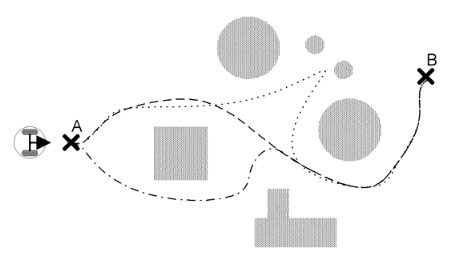
\includegraphics[scale=.5]{./Figures/trayectorias_posibles.png}
	\caption{Algunas de las posibles trayectorias que podría adoptar el robot móvil.}
	\label{fig:trayectoriasPosibles}
\end{figure}

%----------------------------------------------------------------------------------------
%	SECTION 2
%----------------------------------------------------------------------------------------

\section{Motivación}

El estudio de la robótica en las universidades de la región se encuentra mayormente avocada a la robótica de manipuladores. Esto tiene sentido desde un punto de vista de oferta y demanda en la industria local, sin embargo, el mercado internacional esta viviendo una fuerte demanda de profesionales capaces de entender y aplicar técnicas de robótica móvil.

Teniendo en cuenta que hasta hace solo un puñado de años atrás, los dispositivos requeridos para llevar a cabo estas tareas hacían que el estudio, desarrollo y aplicación de tareas de robótica móvil sean extremadamente costosos, aún a pequeña escala, la realidad actual es diferente. Hoy, y gracias a la masificación de ciertas tecnologías, es posible armarse de toda una gama de sensores, actuadores y sistemas capaces de procesar el flujo de datos requerido para estas aplicaciones con muy poco dinero, en muchos casos reutilizando componentes originalmente destinados a otros propósitos.

Aún con la importante reducción de precios vivida en los últimos años, las plantas de prueba ofrecidas por empresas internacionales para fines didácticos continúan siendo prohibitivas para muchas instituciones educativas, así como también para la mayoría de los estudiantes. Es por esto que el presente trabajo se desarrolla en torno a la propuesta de planta de pruebas para el estudio y aplicación de técnicas de robótica móvil. Esta propuesta se centra en dos restricciones importantes, bajo costo y disponibilidad en el mercado local.

%----------------------------------------------------------------------------------------
%	SECTION 3
%----------------------------------------------------------------------------------------

\section{Descripción de tecnologías}

Blabla.

%----------------------------------------------------------------------------------------
%	SECTION 4
%----------------------------------------------------------------------------------------

\section{Objetivos y alcance}

Blabla.
